% Arshad Ansari
\documentclass[12pt]{book}
\usepackage{fontspec}
\usepackage{polyglossia}
\usepackage[T1]{fontenc}
%\usepackage{fontenc}
\usepackage[utf8]{inputenc}
\usepackage{anyfontsize}
\usepackage{mathptmx}
\usepackage{graphicx}
\usepackage[margin=3cm]{geometry}
\usepackage{mdwlist}
\usepackage{longtable}
\usepackage{mathtools}
\usepackage{float}
\usepackage{ragged2e}
\usepackage[backend=biber]{biblatex}
\addbibresource{report.bib}

\newfontfamily\englishfont{Times New Roman}
\newfontfamily\devanagarifont[Script=Devanagari]{Lohit Devanagari}

\graphicspath{ {figures/} }

\restylefloat{figure}

\setmainlanguage{english}
\setotherlanguages{sanskrit}

\begin{document}
\pagenumbering{gobble}
\newgeometry{left=3cm,top=2cm, bottom=0.1cm}
% Front Cover page
\thispagestyle{empty}

\begin{center}
    \noindent \hfill \textbf{Roll No.:} ----------------\\
    \noindent \hfill \textbf{Date of presentation:} ----------------\\
    \noindent \hfill \textbf{SEM/Stage:} III / I \\
  	\fontsize{20}{30}\selectfont \textbf{Sentiment Analysis of transliterated
        hindi and marathi script}\\
  	\fontsize{16}{30}\selectfont \textbf{DISSERTATION SEMINAR}\\
  	\fontsize{14}{24}\selectfont Submitted in partial requirement for the degree of\\
  	\fontsize{16}{30}\selectfont \textbf{Master of Engineering}\\
  	\fontsize{14}{30}\selectfont \textbf{Information Technology (AI and Robotics)} \\
  	by\\
  	\textbf{Mr. Mohammed Arshad Ansari}\\
    \textbf{\underline{Dissertation Guide}}\\
  	\textbf{Prof. Sharvari Govilkar}\\
    (Asst. Prof. Computer Department)\\
	\vspace{30mm}
	\begin{figure}[ht!]
	  \centering
	  
\includegraphics[width=30mm]{piit.png}
	\end{figure}
  	\fontsize{14}{20}\selectfont \textbf{DEPARTMENT OF INFORMATION TECHNOLOGY\\PILLAI INSTITUTE OF INFORMATION TECHNOLOGY,\\
	ENGINEERING, MEDIA STUDIES \& RESEARCH\\ NEW PANVEL - 410206\\UNIVERSITY OF
    MUMBAI\\Academic Year 2015-16}

\end{center}

% Certificate page
\newpage
\begin{left}
    \begin{center}
        \fontsize{12}{30}\selectfont \textbf{\underline{SENTIMENT ANALYSIS OF
            TRANSLITERATED HINDI AND MARATHI SCRIPT}}\\
        \fontsize{12}{30}\selectfont \textit{submitted in partial requirement for
        the degree of Masters in Engineering for Information Technology (AI and
        Robotics by,)}\\
    \end{center}
    \vspace{10mm}
    \noindent ---------------------------------------\\
    \fontsize{12}{30}\selectfont \textbf{(Mr. Mohammed Arshad Ansari)}\\
    \fontsize{12}{30}\selectfont \textbf{(Student)}\\
    \noindent ---------------------------------------\\
    \fontsize{12}{30}\selectfont \textbf{(Prof. Sharvari Govilkar)}\\
    \fontsize{12}{30}\selectfont \textbf{(Project Guide)}\\
    \vspace{10mm}
    \begin{center}
    \fontsize{12}{30}\selectfont \textbf{Examiners} \\
    \noindent ---------------------------------------\\
    \noindent ---------------------------------------\\
    \noindent ---------------------------------------\\
    \noindent ---------------------------------------\\
    \noindent ---------------------------------------\\
    \vspace{10mm}
    \end{center}
    \noindent ---------------------------------------\\
    \fontsize{12}{30}\selectfont \textbf{(Head of Department)} \\

\end{left}
\restoregeometry

% Acknowledgement page
\newpage
\begin{center}

	\vspace{30mm}
    \fontsize{24}{60}\selectfont \textbf{Acknowledgement}\\
    \vspace{20mm}

		
	\fontsize{12}{20}\selectfont \justifying{I am using this opportunity to
        express my gratitude to everyone who supported me throughout the course
        of my time in ME. I am thankful for their aspiring guidance, invaluably
        constructive criticism and friendy advice during the work. I am
        sincerely grateful to them for sharing their truthful and illuminating
        views on a number of issues related to the project.}\par\\
    \vspace{10mm}
	\fontsize{12}{20}\selectfont \justifying{I express my warm thanks to our
        HOD, Dr . Madhumita Chatterjee for her support, consideration and guidance. Finally, a special thanks and humble appreciation of my project guide, Mrs.
    Sharvari Govilkar for making this happen. Her guidance, support and vision
    is what enabled this work and will enable what follows after this.}\par \\
    \vspace{10mm}
	\fontsize{12}{20}\selectfont \justifying{I would also like to thank all the people who provided me with the
    facilities being required and conductive conditions for my ME stage one
    presentation.}\par
    \vspace{70mm}
    \noindent\hfill \fontsize{14}{20}\selectfont -----------------------------\\
    \noindent.\hfill \fontsize{14}{20}\selectfont Mohammed Arshad Ansari\\
\end{center}
\newpage
\begin{center}
  \vspace{30mm}
  \fontsize{24}{60}\selectfont \textbf{Abstract}\\
  \vspace{20mm}

    \fontsize{12}{20}\selectfont \justifying{There is a growing research on
        sentiment analysis of various languages, which is being supplanted
        heavily by those same techniques and methods being applied on the mix
        code or transliterated text for the same purpose. This growing research
        is a result of necessity created through the advent of social media as
        well as textual analysis of the data being collected online. This
        paper, rather than being a pioneer, is about extending that research
        for further improvement. Herein, we assess the existing status,
        standards and achievements of the researchers in the given field and
        supplant it with out proposed methology to increase precision.}\par\\
	\vspace{10mm}
    \fontsize{12}{20}\selectfont \justifying{Although, the current work is a
        proposal with improvements over established techniques, it is also
        however gonig to be quite comparative when it comes to the existing
        findings. The idea is to not just improve what has already been built
        or shown to be true, but also check if the simplest approach is still
        the best way to proceed or not. By this we mean the existing direct
        supervised learning for sentiment analysis, without much NLP or
        language specific work.}\par\\
	\vspace{10mm}
    \fontsize{12}{20}\selectfont \justifying{Since we shall be testing our
        approach against the existing state of the art as well as entering the
    area previously not under coverge (marathi transliterated text), this work
is bound to make great strides in the field of sentiment analysis.}\par\\


\end{center}


\tableofcontents

\addcontentsline{toc}{chapter}{i. List of Figures}
\listoffigures

\addcontentsline{toc}{chapter}{ii. List of Tables}
\listoftables

\clearpage

\pagenumbering{arabic}

\chapter{Introduction}

\paragraph
Sentiment analysis is a process of analysing natural language and figuring out
the sentiments involved or expressed through the source material, with respect
to the topic. The basic idea behind sentiment analysis is that each textual
sentence may or may not contain some kind of polarity, expressing a degree of
emotions along with the information. It is much easier to read in to those
polarity when the text is spoken and not written due to the tone of the
speaker; whereas, in case of written text, it is the context that is useful
while determining the polarities in the statements. Sentiment analysis has
grown to be one of the most important research areas when it comes to textual
analysis on the web. Reason being, obviously, is to be able to make sense of
the data as well as to understand the tone of information being provided. There
are numerous application, ranging from product/customer support review to
improve quality of service (QOS) by corporations to understanding geo-political
motivations when certain news breaks. People react on social media, especially
when they are charged emotionally and when emotions take the form of textual
content to vent, it has been observed that it does in a manner which is more
close to a person's mother tongue.\\


Hindi is spoken by more than 500 million people around the world, making it one
of the most spoken language in the world. Besides, English has turned out to be
an international language, a lot of people speak English on the internet,
however; as described above, there are instances when people use english
language to phonetize and express in a foreign language. This is seen far more
in India subcontinent, where people prefer to write using english alphabets,
but most often, use the words from the mother tongue. If we only look at all
the youtube comments (especially if they are about some controversial issues),
we would see a lot of usage of such transliterated messages or mix-script
writing. Another behavior worth noting is related to vocabulary. People from
subcontinent use words such as 'Bye', 'Thank you', 'Good night', 'Please',
'Sorry' and intermix them with their native tongues. This mixture of language
has been observed profoundly at varying levels of society. Therefore, it would
not be very far-fetched to say that the languages are evolving by mixing
language themselves. This forms the necessary reason for why there needs to be
analysis of mixed-languages and it starts with analyzing that which is mostly
available, the mixed-script. Here, we are not going to invent something new,
nor are we going to do something entirely differently. However, the purpose
behind this work is to stand on the shoulders of giants and take the research
of what has already been done to what it can be. This we strive to do, by
improving the performances by innovatively applying techniques which have
worked better in other cases. Therefore, as it will be seen, our proposed
approach as well is a mixture of disparate attempts in varying domains (even
slightly) to come together for better whole.\\

Sentiment analysis is a lot tougher for languages that are outside eurozone,
due to their lexical syntax being very different from european languages as
well as due to majorly, less amount of work being done on it. Semantic analysis
requires annotated text corpus to train classifers, which is most of the time a
very huge manual task. It has been undertaken for English and for many other
European langauges, while at the same time, work from one supplementing work
for another language, due to the similarities existent in those languages. When
it comes to languages such as Hindi and Marathi, such resources are very less
compared to the above mentioned languages. Moreso for Marathi, since a lot of
work has been done and progress made in case of Hindi. Most of the reason for
the under development of the research for these languages are (1) Not much
annotated textual corpus needed for traning, (2) Lack of basic language tools
like taggers and parsers. These problems will be solved in time and this work
is a part of all the woks which will finally solve this problem. 
Having expressed the problem, in this work, we also laude the work that has
already gone in to this respective field, without which this would not have
been possible. It is really interesting to note, that a great amount of effort
has just started pouring in for this particular part of sentiment analysis. It
is naught with great anticipation that this work is being progressed. Besides,
as the sentiment analysis of the textual data being to shape more and more, the
greater the benefit will be to the field of general AI. When it comes to human
capacity, not representing emotions would be the biggest gap in the domain,
which exactly is sentiment analysis has started to fill. \\


\chapter{Motivation}

\paragraph
We can discuss two kinds of motivation herein, one being in general about
sentiment analysis and the other a bit specific about this very work itself.
Sentiment analysis has tons of applications, especially in the current era of
social media. The entire planet's population is connecting with one another and
learning about each other's cultures and assimilating ideas from one another
and then followed by sharing ideas, concerns and assaults on the social media.
Whatever may be the case, all the information being transferred is textual in
nature. It becomes of vital import that the sentimental exchanges happening on
such channel is being monitored. For example, twitter and facebook led to the
entire arab world to be engulfed in flames. The previous example was just to
elaborate how the social media and in extension written media, with the
emotional content, can literally change the world. Having understood the
important, let's look at many possible applications for sentiment analysis.\\
\begin{itemize*}
  \item \textbf{\textit{Product / Service Review}}; Product here can extend
      from movies, daily usage products to books, etc. They are usually
      reviewed either on social media or sites dedicated to such reviews.
      Examples being Amazon, Google/Iphone App store, Good Reads, etc. These
      reviews allows other users to decide whether they want to buy reviewed
      product or not. Similary, service providers like ISP, Telecom providers,
      etc are interested in review of the service they are providing, including
      customer service reviews. These reviews help the providers to improve the
      service by addressing the negetive aspects and focusing more on postive
      ones. \\
  \item \textbf{\textit{Discourse Analysis}} on topics that range from
      philosophical to wars between countries are also candidates for such
      analysis. It becomes really important when taking decisions whether the
      debate pertaining to such decisions are emanating from emotions or
      logically grounded arguments. \\
  \item \textbf{\textit{Feedback Analysis}} for teacher's from students or
      about government from population. They all have one thing in common, that
      is, they are all textual and by extension is candidate for sentiment
      analysis. \\
  \item \textbf{\textit{Other areas}}: such as emails analysis,
      twitter/facebook feed analysis or blog analysis, help in understanding
      the emotions of authors regarding the topics, which help focus on
      problems, which can be the cause of negetive emotions. \\
\end{itemize*}

 Above being the motivation for sentiment analysis in general, let's consider the motivation for this specific work. As explained in introduction as well as in the above listed areas of interest; where the source is always textual data, this data usually consists of mixed script in terms of language. That being the what, let's look at why. And more specifically why Hindi and Marathi. Marathi by itself is playing catch with Hindi, where Hindi language is making strides in this research. Although there aren't many marathi speakers in comparison to hindi itself, but it is still spoken by million of people in the region of Maharashtra, which by the way has a lot of literature that has yet to be digitized and benefit the world with it. The real reason is the aspect of completion. Many terms like 'Layi Bhari' and many other slangs have crept from Marathi to Hindi and then taken to the country as whole through bollywood movies. Many inside jokes in many bollywood movies have their roots in marathi language and regional aspects. These will never be easily covered if marathi itself doesn't become partial focus of the research itself. Although, there are very few input sources to consider for marathi, there still exists some, in form of youtube comments, etc, which can be part of this research. Going back to hindi itself, a lot of textual resource considers mixed script statements as noise, which definitely contains gold from sentiment analysis perspective. And, therefore, we have decided to augment the existing research by improving the precision where research is being performed and pave the way where the research is still lagging behind.

\chapter{Literature Review}

\section{Related Work}

\subsection{Code Mixing and Transliteration}

Code mixing has been done for more than a couple decades and was investigated
during initial period by Gold \cite{gold_language_1967} for the purpose of
language identification. The same phenomenon for Indian langauges was worked
upon by Annamalai \cite{annamalai_anglicized_1978}, pioneering the research
field for the subcontinent languages. Recently, it was investigated by Elfarti
et. al. \cite{elfardy_token_2012} and was termed as linguistic code switching
by the research group. Karimi \cite{karimi_machine_2011} made the case for
machine translation for the purpose of transliteration in the survey and
suggested transliteration based on phoneme based approach and transliteration
generation using bilingual corpus, while presenting the key issues that arise
during the transliteration process. Dewaele \cite{dewaele_emotions_2010}
pointed out the strong emotional presence as being the main marker for the
existence of code switch that happens in textual corpus. Gupta et. al.
\cite{gupta_mining_2012} mined the tranlisteration pairs between hindi and
english from the music lyrics of bollywood songs for Fire'14 shared task, which
is quite handy for training in language sentiments. 

\subsection{Language Identification}
The issue of identification of language of the code - mix script is another
challenge that has been answered by the research community. A statistical
approach was proposed by Kundu and Chandra et. al. \cite{kundu_automatic_2012}
for the automatic detection of English words in Bengali + English (Benglish)
text. A conditional random field model for weakly supervised learning model was
used for word/token labelling by King and Abney \cite{king_labeling_2013} with
a good result of > 90\%. Barman \cite{barman_code_2014} used facebook user data
for identifying the language in mixed script and concluded that the supervised
learning outperforms the dictionary based approaches. POS Tagging and
transliteration efforts for Hindi + English data on social media was
experimented upon by Vyas et. al. \cite{vyas_pos_2014} and came to the
conclusion that any operation on transliteration text will largely benefit from
pos tagging. 

\subsection{Sentiment Analysis}
Although sentiment analysis is being worked upon for quite some time now and it
has already entered the mainstream application. There are works being done
transliteration of Indian languages, out of which some have been listed below
under this section.\\

Joshi et.al. \cite{joshi_fall-back_2010} performed experiment to compare three
approaches for the sentiment analysis of hindi text and found that HSWN
performs better than Machine Translation approach but under performs in
language traning of sentiment corpus in hindi. This was, however; performed in
2010 and the HSWN has been continually improving past these experiments. The
same result was reiterated with by Balamurali et. al.
\cite{hutchison_lost_2013}. Kashyap \cite{kashyap_hindi_????} found a way to
perform Hindi Word Sense Disambiguation using wordnet with encouraging results
for nouns. Subjective lexical resource was developed by Bakliwal et. al.
\cite{bakliwal_hindi_2012} by using only wordnet and graph traversal algorithm
for adverbs and adjectives.\\

Balamurali A R et. al. \cite{balamurali_a_r_cross-lingual_????} performed
experiement to figure out in language supervised training of sentiments against
the machine translated source for sentiment analysis. They found that the MT
based approach under performs much worse compared to in language traning of
sentiment. Fuzzy Logic membership function was used to determine the degree of
polarity of the sentiment for a given POS tagged preposition by Rana
\cite{shweta_rana_sentiment_2014}. Hindi Senti WordNet was developed by
Balamurali A. R. et. al. \cite{balamurali_a_r_cross-lingual_????} using the Senti Wordnet by using linked wordnet. HSWN along with negetion discourse was applied by Pandey
\cite{pandey_framework_2015} and Mittal et. al. \cite{mittal_sentiment_2013} or
sentiment analysis of Hindi language text corpora, with the accuracy of 80.21
achived. \\

\subsection{Sentiment Analysis of code mix}
There is only one work done on the sentiment analysis of hindi transliteration
by Srinivas (\cite{sharma_text_2015} and \cite{shashank_sharma_sentiment_????}
) and the approach taken was to tag words with identified language and then run
against respective POS tagger for languages and sentiment analysis done on the
output. The approach yielded 85\% percision. Although not much has been done on
marathi front, however; it is still in the works and pipeline.\\

\section{Literature used for proposed approach}

As shown in table \ref{tab:tab1}, these works have heavily
influenced the proposal and are the one of the few works done on the subject.\\

\begin{longtable}[c]{ |p{3cm}|p{3cm}|p{3cm}|p{3cm}|p{3cm}|  }
  \hline
  Paper & Author & Approach & Result & Limitation\\
  \hline
  \endhead
  Hindi subjective lexicon: A lexical resource for hindi poliarty
  classification \cite{bakliwal_hindi_2012} & Bakliwal, Akshat, Piyush Arora ad Vasudev Varma & Usage of
  sense based sentiment analysis and devlopment of HSWN& Resource for hindi &
  Doesn't work on transliteration of hindi text\\ 
  \hline
  A framework for sentiment analysis in hindi using HSWN
  \cite{pandey_framework_2015} & Pooja Pandey , Sharvari Govilkar & Devnagiri
  sentiment analysis using HWSN
  and use of negation discourse analysis & Usage of negation and discourse
  analyse improves the result of polarity detection & Doesn't work with hindi
  transliteration\\
  \hline
  Automatic Detection of English words in Benglish text: A statistical approach
  \cite{kundu_automatic_2012} & Kundu, Bijoy and Chandra, Swarup & Statistical
  method developed which is language independent and can be used to detect any
  foreign language. & Accuracy upto nearly 72 percent. & There is a great scope
  of increasing the accuracy by improving methodology.\\
  \hline
  Sentiment Analysis of Hindi Review based on negation and discourse relation
  \cite{mittal_sentiment_2013} & Namita Mittal, Basant Agwarwal, Garvit Chouhan
  and Nitin Bania & Negation and discourse relation were identified and HSWN
  improvement carried out & Accuracy upto nearly 81 percent & Transliteration
  not covered. Scope for accuracy improvement.\\
  \hline
  Text Normalization of Code Mix and Sentiment Analysis \cite{sharma_text_2015} & PYKL Sriniva and
  Shashank Sharma & Language identification and transliteration to devnagiri
  script and then using HSWN for sentiment analysis.& Accuracy upto 85 precent
  & Negation and discourse analysis not being performed. \\ 
  \hline

  \caption{Papers that forumulated the approach}\label{tab:tab1}\\
\end{longtable}


\chapter{Proposed Approach}

\section{Problem Statement}

\textit{The proposed work is geared towards the problem of sentiment analysis
    of code - mix script (Romanized) for languages such as hindi and marathi.
    The current literature has brought the accuracy up to 85 percent for hindi
    transliterated text, which this work aims to take to 90-95 percent accuracy
    and paritially accomplish for marathi language as well.}


\section{Scope of work}

The current word considers hindi/marathi text in romanized script as input
which may contain phonetic words, sounds; however, it is not considering social
language like gr8, rt, f9, etc as input source. For now it is considered as
noise for the result of this work. Although, we are not performing sentiment
analysis on English text as part of this text, which is simply because it has
been under taken in many works preceeding this one. Therefore, concentration
will solely be on the text which is transliterated hindi or marathi. Also, the
architecture of proposed approach has intergration in mind and hence, it will
be able to plug social sentiment analysis or twitter sentiment analysis or
plain english analysis and will work only for the transliterated text, while
taking inputs from the mentioned analyzers for their established polarity. The
results can be merged and shown to have improved the overall accuracy. 


\section{System Architecture}

There are going to me multiple approach for testing to be implemented as part
of this work. The purpose of those work will be to ensure that the proposed
system performs better than what has been accomplished by other researchers.
Although, here we will only go into the actual proposed system to understand
its working and predict the possible improvements.
The proposed approach we are to take in this work comprises of extending the
work of Srinivas \cite{shashank_sharma_sentiment_????} with multiple
improvement points at multiple level of the process. Each step is listed below
with the improvement suggested from this work. All the work done on that paper
has been uploaded to the website \cite{_linguistic_????}, which we shall be
using in this paper extensively and building on top of it. 

\begin{figure}[ht!]
    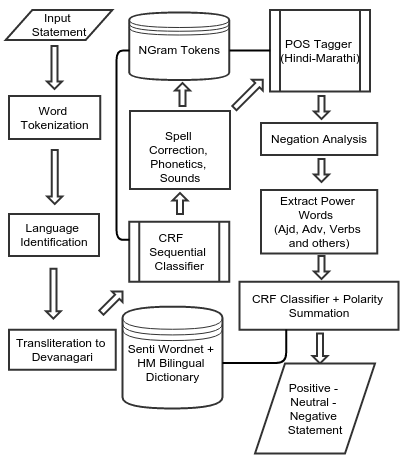
\includegraphics[width=140mm]{polarity-pickup.png}
    \caption{Flow diagram for the proposed approach}
\end{figure}


\subsection{Text Normalization}
Text normaliation step depends heavily on work of Srinivas
(\cite{sharma_text_2015}), which has following steps:
\begin{itemize*}
  \item \textbf{\textit{Language Identification}}; Tagging of the words as
      <word>/<tag>, where <tag> can be E or english, H for hindi and M or
      marathi,\\
  \item \textbf{\textit{Spelling Corrections}}; There are multipe ways to write
      Mujhe in hindi such as muze, muje, etc. To come to common and widely used
      spelling becomes very importnat\\
  \item \textbf{\textit{Ambiguous words}}; Words such as 'me' means same thing
      in english and marathi, where as in hindi it is sometimes used to say
      inside with another spelling being 'mein'. \\
  \item \textbf{\textit{Sounds}}; Words such as aww, oohh, ouch, ewww, etc.
      They do contain rich information when it comes to sentiments.\\
  \item \textbf{\textit{Phonetic words}}; Words such as pleej usually is
      misspelling of word please, spoken in some areas of the subcontinent. It
      gets written too in the similar manner.\\
  \item \textbf{\textit{Transliteration}}; Conversion of hindi/marathi words
      written in english to appropriate devnagari script.\\
\end{itemize*}

All then above enumerated steps have been covered by Srinivas
(\cite{sharma_text_2015}) and doesn't require us to go in the details of those,
however; we will look at some of those steps to get a proper grip on the
subject. At this point, this work will simply reuse those steps for hindi and try to
closely perform them for marathi as well. 

\subsubsection{Work-Token Normalization}
The process here is really simple to explain, but quite interesting to develop.
This is a required step as a sort of preprocessor, to enable the words to be
converted appropriately to their respective languages. Words like "awww",
"reaaaly", etc needs to be normalized and the techniques to do are covered by
Srinivas (\cite{sharma_text_2015} and \cite{shashank_sharma_sentiment_????}
) both. These methods are already tested with some accuracy in the above
mentioned papers themselves.  

\subsubsection{Language Identification Tagging}
The first step is to tag the language identifier for every word-token, using the techniques described in Kundu and Chandra et. al.
\cite{kundu_automatic_2012} and King and Abney \cite{king_labeling_2013}. The
output of this step will be more or less like in example given below:\\

\hspace{8em}"Yeh acchha din hai. Let's go now" \\
\hspace{8em}"Yeh|H acchha|H din|H hai|H. Let's|E go|E now|E". \\
To this effect, same approach can be accomplished for marathi text. Once we have tagged all the
word-tokens with their corresponding language identifier, we can move to next
step. However, there are going to be ambigious words "ho", "me", etc, which
shall use semi supervised learning for handing based on context. The plan is to
also test again HMM models to discover the accuracy difference.\\

Language identification will be based on the approach of using hidden markov
models trained on the n-gram generated from corpus to be able to produce
probabilities for each work-token when considered with its neighbouring words
to identify the language to which the token belongs.\\

In all the related work \cite{shashank_sharma_sentiment_????}, there was a need
for transliteration mechanism in play on the fly. The reason for it being the
de facto method of choice is because it allows the usage of POS tagging to work
with the text, which would only \\
This database will be trained using hindi-english transliteration pairs
collected from Fire 2013 found at \cite{_linguistic_????} as well as result
of another previous work by Gupta et. al. \cite{gupta_mining_2012}. This
trained model will then be used to convert all the words in hindi wordnet to
ensure greater coverage of incoming input word tokens. In case of marathi, a
similar thing will be done and associated with hindi wordnet through
hindi-marathi bilingual dictionary.\\ 

\subsubsection{POS Tagging, Discourse analysis, Senti Word Net}
Before sentiment analysis can be performed, it is necessary to deal with few
important things. We are striving to extend and improve upon earlier work such
as Srinivas (\cite{sharma_text_2015}) and therefore following much in the same
footsteps. Both the step are explained further below.
Once we have the document in english or hindi, the next step is to run it
through POS tagger based on respective language. The approach will be straight
forward as detailed here \cite{vyas_pos_2014}. The POS Tagged prepositions
then shall be run through the negation discourse analysis to invert the POS
tagged adjectives and adverbs in case of negetive discourse as explained by Pandey
\cite{pandey_framework_2015} and Mittal et. al. \cite{mittal_sentiment_2013}.
The output of POS Tagger shall be used to look up sentiword identifier for the
word groups using Sentiwordnet or HSWN, for English and Hindi, respectively.
HSWN has been improved by Pandey \cite{pandey_framework_2015} by making
additions to it and that will be used in this work. Here, there are three major
improvements we are considering. Since, it was established
\cite{shashank_sharma_sentiment_????} that the basis for sentiment analysis
being POS tagged adjectives and adverbs gives much better result that depending
direcly on lexicon or wordnet look up for each work, we would be going that
route. Secondly, addition of discourse analysis would further enhance on the
existing work \cite{shashank_sharma_sentiment_????}.

\subsubsection{Sentiment classification using classifier}
Once we get sentiword identifier for each token - word, next step is to put it
through the classifier which will give the polartiy of the statement provided.
This polarity checking decision can be as simple as simple summation of all
word-token sentiment polarities or further analysis can be performed to figure
out what really is the polarity of word-token and its membership with negetive,
postive or neutral . This step being the vital one can be accomplished using
most trust classifier like SVM, Random Forests, however; impetus shall be given
on naive bayes classifier for brevity's sake. \\
Quite clearly, we have input as POS tagged statements with greater emphasis on
adjectives and adverbs that are inverted in case of negation present in the
preposition. Once we have this tagged information, we would like to test on
both the process of simple polarity count summation of the given input and
traning the classifier, in order to come up with the best possible result in
terms of accuracy.\\

\subsubsection{\textbf\textunderline{Example flow}}
\textbf{\textit{Input:}} \\
Kitni der se ticket cancel nahi ho rahi hai\\
\textbf{\textit{Language Identification:}}\\
kitni|H der|H se|H ticket|E cancel|E nahi|H ho|H rahi|H hai|H\\
\textbf{\textit{Transliteration:}} \\
\foreignlanguage{sanskrit}{
कितनी देर से
}
ticket cancel
\foreignlanguage{sanskrit}{
नहीं हो रही है  
}\\
\textbf{\textit{POS Hindi:}}\\
\hspace{20em}\foreignlanguage{sanskrit}{कितनी}|adj - QF\\
\hspace{20em}\foreignlanguage{sanskrit}{देर}|adv - NN\\
\hspace{20em}\foreignlanguage{sanskrit}{से}|v - PSP\\
\hspace{20em}ticket|unk - JJ\\
\hspace{20em}cancel|unk - NN\\
\hspace{20em}\foreignlanguage{sanskrit}{नहीं}|adv - NEG\\
\hspace{20em}\foreignlanguage{sanskrit}{हो}|v - VM\\
\hspace{20em}\foreignlanguage{sanskrit}{रही}|v - VAUX\\
\hspace{20em}\foreignlanguage{sanskrit}{है}|v - VAUX\\
\\
\textbf{\textit{Negation discourse analysis:}} \\
\foreignlanguage{sanskrit}{नहीं} and \foreignlanguage{sanskrit}{हो} are closely
associated with one another. Negation discourse analysis works on the subtree
level, which in this case is post the word \foreignlanguage{sanskrit}{हो} a. \\
So all the words following 'nahi' will be part of it's subtree. Hence, all the
polarity from that point onwards will be reverse.

\textbf{\textit{Poliarity extraction example:}} 
\hspace{20em}= \foreignlanguage{sanskrit}{कितनी}|adj=INC
\foreignlanguage{sanskrit}{देर}|adv=NEG \foreignlanguage{sanskrit}{से}|v=NEU
ticket|NN=Neu cancel|=NEG \foreignlanguage{sanskrit}{नहीं}|adv=NEG
\foreignlanguage{sanskrit}{हो}|v=NEU  \foreignlanguage{sanskrit}{रही}|v=NEU
\foreignlanguage{sanskrit}{है}|v=NEU\\ 
\hspace{20em}= (INC * NEG) + NEU + NEG + [NEG:REVERSE + NEU + NEU + NEU]\\
\hspace{20em}= (2 * -1) + 0 + -1 + (-1 * (0 + 0 + 0))\\
\hspace{20em}= -2 + 0 -1 + (-1 * 0)\\
\hspace{20em}= -2 -1 + 0\\
\hspace{20em}= -3\\

Here the numbers picked up are in unit but they will be from the polarity
values directly from senti wordnet.


\subsection{Algorithms for proposed approach}

Following are the list of all the algorithms that will be required for this
propsed approach

\subsubsection{Algorithm for language identification}
Algorithm to tag words with language identifier with spelling corrections

\begin{longtable}[c]{ |p{16cm}|  }
  \hline
  \textbf{Algorithm steps} \\
  \hline
  \endhead
  \textbf{\textit{Arguments}} \\
  \hline
  w : word to identify language for\\
  sentence : sentence to which word belongs\\
  \hline
  \textbf{Variables and methods} : list of variables and methods \\
  \hline
  Le : Text corpus in english language\\
  Lh : Text corpus in hindi language\\
  Lm : Text corpus in marathi language\\
  Qeh:  Hindi Devnagiri to Latin Script transliterator\\
  Qem:  Marathi Devnagiri to Latin Script transliterator\\
  Leh:  Transliterated Hindi Corpus\\
  Lem:  Transliterated Marathi Corpus\\
  FNGram:  Algorithm to get n-grams from sentence\\
  % HMM:  Hidden markov models\\
  CRF:  Conditional Random Field\\
  D:  Language dictionary\\
  l:  Language Tag\\
  \hline
  if Leh is None:\\
  \hspace{4em}Leh = Qeh(Lh{i}) for i in Lh\\
  if Lem is None:\\
  \hspace{4em} Lem = Qem(Lm{i}) for i in Lm\\
    
  if not model:\\
  \hspace{4em}Model = CRF(FNGram(Leh), FNGram(Lem), FNGram(Le))\\
  \hspace{4em}if not w in D: \\
  \hspace{8em}w = stem word(w)\\
  \hspace{12em}if w not in D:\\
  \hspace{16em}w = find most similar word(D, w)\\
  l = arg max(Model, sentence, w)\\
  return l\\
  \hline
  \caption{ Algorithm: Language Identifier }\label{tab:tab_language_identifier}\\
\end{longtable}

\subsubsection{Algorithm for pos tagged with negetation}
Algorithm to pos tag words with negetation\\

\begin{longtable}[c]{ |p{16cm}|  }
  \hline
  \textbf{Algorithm steps} \\
  \hline
  \endhead
  \textbf{\textit{Arguments}} \\
  \hline
  sentence : sentence to which word belongs\\
  \hline
  if max(tags in sentence) is english:\\
  \hspace{4em}TaggedSentence = POSTaggerEnglish(sentence)\\
  else max(tags in sentence) is hindi:\\
  \hspace{4em}TaggedSentence = POSTaggerHindi(sentence)\\
  return replace negetive phrases with antonyms(TaggedSentence)\\
  \hline
  \caption{ Algorithm: POS Tagged With Negetation}\label{tab:tab_pos_tagger}\\
\end{longtable}

\subsubsection{Algorithm for polarity identification}
Algorithm for polarity identification\\

\begin{longtable}[c]{ |p{16cm}|  }
  \hline
  \textbf{Algorithm steps} \\
  \hline
  \endhead
  \textbf{\textit{Arguments}} \\
  \hline
  sentence : sentence to which word belongs\\
  \hline
  languageTaggedSentence = (LanguageIdentifier(sentence, word) for word in sentence).join(' ')\\
  posTaggedSentence = POSTag(languageTaggedSentence)\\
  polarWords = extractAdjectivesAdverbs(posTaggedSentence)\\
  wordPolarity = dict()\\
  for word in polarWords:\\
  \hspace{4em}if word tagged as english:\\
  \hspace{8em}wordPolarity[word] = sentiwordnetPolarity(word)\\
  \hspace{4em}elif word tagged as hindi:\\
  \hspace{8em}wordPolarity[word] = hindiSentiwordnetPolarity(word)\\
  \hspace{4em}else:\\
  \hspace{8em}hindiWword = hindiMarathiBilingualDictionary(word)\\
  \hspace{8em}wordPolarity[hindiWord] = hindiSentiwordnetPolarity(hindiWord)\\
  return wordPolarity\\
  \hline

  \caption{ Algorithm: Polarity Identification}\label{tab:tab_polarity_identifier}\\
\end{longtable}

\subsubsection{Algorithm to classify polarity}
Algorithm for classify polarity using naive bayes classifer as well as simple linear summation.\\
We can add more algorithms here for comparison

\begin{longtable}[c]{ |p{16cm}|  }
  \hline
  \textbf{Algorithm steps} \\
  \hline
  \endhead
  \textbf{\textit{Arguments}} \\
  \hline
  sentence : sentence to which word belongs\\
  \hline
  \textbf{\textit{Variables and methods}} \\
  \hline
  NaiveBayesClassifier -> Trained to return polarity of the entire sentence given tokens with polarity values\\
  LinearCalculation -> Simple Summation based polarity classifier\\
  \hline

  wordDictionary = PolarityIndentification(sentence)\\
  return NaiveBayesClassifier(wordDictionary), LinearCalculation(wordDictionary)\\
  \hline

  \caption{ Algorithm: Polarity Classification}\label{tab:tab_polarity_classifer}\\
\end{longtable}



\chapter{Application}

As suggested in the motivation, there are two ways this work can be applied,
one being about sentiment analysis in general and the other regarding sentiment
analysis of transliterated text to be specific. We shall focus on the latter
aspect. 


\begin{itemize*}
  \item \textbf{\textit{Product / Service Review}}; Figuring out the polarity
      of general public in form of reviews is common using sentiment analysis,
      however, adding transliteration to the mix had made it very difficult
      thing to achieve. This way, the said text will not act as noise and will
      rather end up becoming much more valuable input.\\
  \item \textbf{\textit{Discourse Analysis}} Once polarity of any discourse and
      / or debate has been established, it becomes easily achievable to take
      decisions based on necessary parameters. Some case are to be treaded
      lightly since it affects a lot of emotions and hence has a direct result
      in public opinion, which as result may affect many future decisions.
      Example at hand can be the intorelance debate going on in the country. Or
      the use of freedom of expression as an excuse to cause mayhem in select
      polity. All of these can be assessed from debates pertaining to the topic
      and considering the emotional impact of the situation.\\
  \item \textbf{\textit{Feedback Analysis}} As explained earlier, feedbacks
      tend to be emotional quite a lot of times and not understanding the
      emotional undercurrent underneath the feedback recieved can be a make or
      break situation for the cause, which required the feedback in the first
      place. Being able to honestly take feedback, without throwing away mixed
      script as noise will shed new light on what feedback are actually
      expressing and result in proper due consideration where it is necessary.\\
  \item \textbf{\textit{Other areas}}: Editorials, Blogs or a media post, each
      have an author, whose non sentiment can be assessed using general idea of
      sentiment analysis. But what more can be done is to analyse the comments
      on those topics and come to consensus of how a certain post is received
      by the audience, who are bound to use their native transliterated text
      for commenting on the topic. 
\end{itemize*}

What is listed above is only tip of the iceberg, there are lot of ways
marketing agencies can use the above infomration for variety of purposes, both
for the benefit of public or otherwise. To be able to read between lines in
such cases again would help take decisions based on right factors than mere
informed gueses.

\chapter{Conclusion}

\section{Future Work}
The most important aspect of this work i.e. the results are what is coming
next. We will show that the approach proposed in this work performs better than
all the work presented here in literature, when considered independently. It is
the synergy, which the approach presented there, promises. The implementation
will happen for all ways that differ from the approach too, so that comparisons
can be made and conclusions drawn without the strawman arguments. 

\section{Remarks}
There is a lot of work to be performed before any concrete conclusion can be
expressed, however; There is a great possibility that the approach suggested in
the given work will result in improvement in the field of sentiment analysis,
that can again be extended for greater language coverage in as well as out of
indian languages. These strides towards such improvements will result in
machine's being able to understand human sentiments better, which is one of the
greatest challenge being faced by the research in general AI. Ours is but a
small step towards that goal. It will not be too far fetched to believe that
the improvements will range from 5 to 10 percent improvement where we will see
the accuracy reach 95 percent. \\



\printbibliography


\end{document}
